\documentclass[class=report, crop=false, 12pt,a4paper]{standalone}
\usepackage{enumitem}
\usepackage{multicol}
\usepackage{graphicx}
\usepackage{float}
\usepackage{amsmath}
\usepackage{amssymb}
\usepackage{mathtools}
\usepackage{siunitx}
\usepackage{commath}
\usepackage{array}
\usepackage{natbib}
\usepackage{tikz}
\usepackage[a4paper,width=150mm,top=25mm,bottom=25mm]{geometry}
\usetikzlibrary{positioning, fit, calc}   
\tikzset{block/.style={draw, thick, text width=3cm ,minimum height=1.3cm, align=center},   
line/.style={-latex}     
}  
\setlength{\parindent}{0pt}
\begin{document}
\section*{Boundary layer theory (Prandtl)}
The flow domain can be subdivided into two parts:
\begin{itemize}
  \item \textbf{Irrotational flow region}, outside of the boundary layer, Bernoulli equation, potential flow and stream function apply
  \item \textbf{Boundary layer} where all vorticity is confined, The friction shear at the airfoil surface acts as a source of vorticity. 
\end{itemize}
\begin{figure}[H]
  \centering
  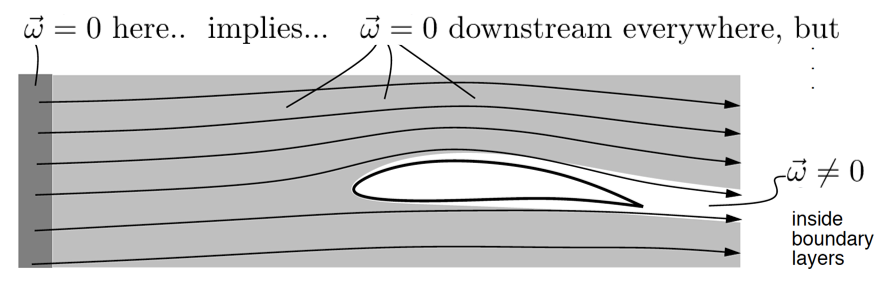
\includegraphics[width = 0.8 \textwidth]{../img/diagram48.png}
\end{figure}
\section{Boundary layer concept}
Immediately adjacent to a solid surface, the fluid particles are slowed by the strong shear force between the fluid particles and the surface. This relatively slower moving layer of fluid is the boundary layer.
\begin{figure}[H]
  \centering
  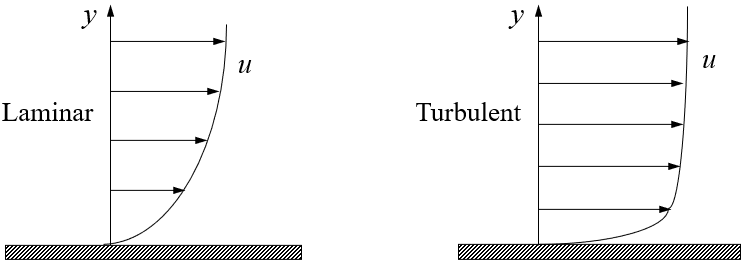
\includegraphics[width = 0.8 \textwidth]{../img/diagram49.png}
  \caption{In turbulent flow, you have a higher shear stress due to the higher velocity close to the boundary. This produces more frictional drag against the motion of the solid surface. ($\tau = \mu \frac{\partial u}{\partial y}$)}
\end{figure}
\section{Boundary layer theory}
Prandtl's concept of the boundary layer in high $Re$ flow is that although viscous forces can be considered small, their effects are not negligible.
\begin{figure}[H]
  \centering
  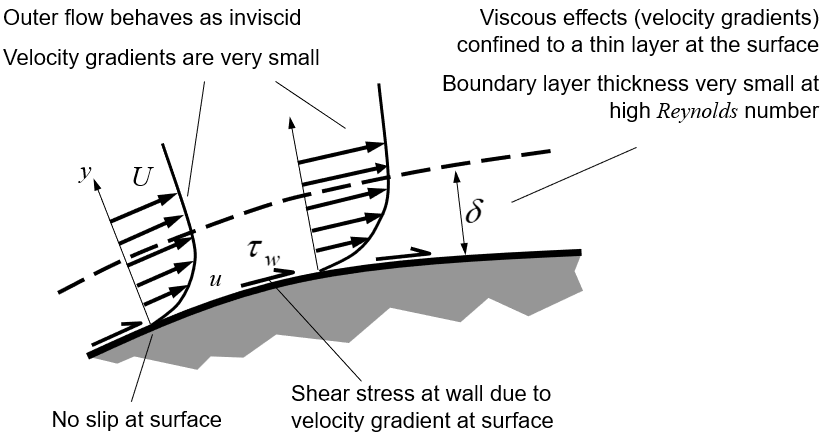
\includegraphics[width = 0.8 \textwidth]{../img/diagram50.png}
\end{figure}
Let us see what happens when we consider the Navier stokes equations for a steady - 2D flow with $Re >> 1$. Continuity equation (conservation of mass):
\begin{align}
  \frac{\partial u}{\partial x} + \frac{\partial v}{\partial y} = 0
\end{align}
Conservation of momentum equations:
\begin{align}
  \textrm{x-direction: } u\frac{\partial u}{\partial x} + v \frac{\partial u }{\partial y} &= - \frac{1}{\rho} \frac{\partial p}{\partial x} + \nu \left(\frac{\partial^2 u}{\partial x^2} + \frac{\partial^2 u}{\partial y^2}\right)\\
  \textrm{y-direction: } u \frac{\partial v}{\partial x} + v\frac{\partial v}{\partial y} &= -\frac{1}{\rho}\frac{\partial p}{\partial x} + \nu \left(\frac{\partial^2 v}{\partial x^2} + \frac{\partial^2 v}{\partial y^2}\right)
\end{align}
Remember that:
\begin{equation}
  Re = \frac{U_\infty L}{\nu}
\end{equation}
Where $L$ is the length of the airfoil being analysed, $U_\infty$ is the velocity of the free stream and $\nu$ the kinematic viscosity. Inside the boundary layer, one thing we can assume that the inertial forces and the viscous forces are comparable, because viscous diffusion is large and of the same order of magnitude of the inertial terms. Therefore:
\begin{align}
  \frac{u\frac{\partial u}{\partial x}}{\nu \frac{\partial^2 u}{\partial y^2}} \approx 1
\end{align}
We need to exploit this relationship in order to derive an expression for $\delta$ in comparison to $L$. Some approximations we can make below are:
\begin{align}
  u &\approx U_\infty\\
  x &\approx L \rightarrow \frac{\partial}{\partial x} \propto \frac{1}{L}\\
  y &\approx \delta \rightarrow \frac{\partial}{\partial y} \propto \frac{1}{\delta}
\end{align}
Combining this with our above assumption:
\begin{align}
  \frac{\frac{U_\infty^2}{L}}{\nu \frac{U_\infty}{\delta^2}} &= \frac{\delta^2}{L^2} Re \approx 1\\
  \delta^2 &= \frac{L^2}{Re}
\end{align}
Looking at the continuity equation:
\begin{align}
  \frac{\partial u}{\partial x} + \frac{\partial v}{\partial y} &= 0\\
  \frac{U_\infty}{L} + \frac{v}{\delta} &= 0\\
  v &= \frac{\delta}{L}U_\infty\\
  v &= \frac{1}{\sqrt{Re}} U_\infty
\end{align}
(signs were ignored). Looking at the momentum equation in the x-direction:
\begin{align}
  u\frac{\partial u}{\partial x} + v \frac{\partial u }{\partial y} &= - \frac{1}{\rho} \frac{\partial p}{\partial x} + \nu \left(\frac{\partial^2 u}{\partial x^2} + \frac{\partial^2 u}{\partial y^2}\right)\\
  \textrm{First term: } u\frac{\partial u}{\partial x} &\propto \frac{U_\infty^2}{L}\\
  \textrm{Second term: } v\frac{\partial u}{\partial y} &\propto \frac{1}{\sqrt{Re}} \frac{U_\infty}{\delta} U_\infty = \frac{U_\infty^2}{\sqrt{Re}} \frac{\sqrt{Re}}{L} = \frac{U_\infty^2}{L}\\
  \textrm{Fourth term: } \nu \frac{\partial^2 u}{\partial x^2} &\propto \nu \frac{U_\infty}{L^2} = \frac{\nu}{L U_\infty} \frac{U_\infty^2}{L} = \frac{1}{Re} \frac{U_\infty^2}{L}\\
  \textrm{Fifth term: } \nu \frac{\partial^2 u}{\partial y^2} &\propto \nu \frac{I_\infty}{\delta^2} = \frac{\nu}{L U_\infty} \frac{U_\infty^2 L}{\delta^2} = \frac{1}{Re} \frac{U_\infty^2 Re}{L} = \frac{U_\infty^2}{L}
\end{align}
We can see in the fourth term that $Re >> 1$, hence it is neglected i.e. there will not be a viscous term due to the variation of the velocity in the x direction w.r.t x. Looking at the momentum equation in the y-direction:
\begin{align}
  u \frac{\partial v}{\partial x} + v\frac{\partial v}{\partial y} &= -\frac{1}{\rho}\frac{\partial p}{\partial x} + \nu \left(\frac{\partial^2 v}{\partial x^2} + \frac{\partial^2 v}{\partial y^2}\right)\\
  \textrm{First term: } u \frac{\partial v}{\partial x} &\propto U_\infty^2\frac{\delta}{L^2} = \frac{1}{\sqrt{Re}}\frac{U_\infty^2}{L}\\
  \textrm{Second term: } v\frac{\partial v}{\partial y} &\propto \frac{U_\infty^2}{L^2} \frac{\delta^2}{\delta} = \frac{1}{\sqrt{Re}} \frac{U_\infty^2}{L}\\
  \textrm{Fourth term: } \nu \frac{\partial^2 v}{\partial x^2} &\propto \nu \frac{U_\infty \delta}{L} \frac{1}{L^2} = \frac{\nu}{L U_\infty} \frac{U_\infty^2 \delta}{L^2} = \frac{1}{Re} \frac{U_\infty^2}{L\sqrt{Re}} = \frac{1}{\sqrt{Re}^3} \frac{U_\infty^2}{L}\\
  \textrm{Fifth term: } \nu \frac{\partial^2 v}{\partial y^2} &\propto \nu \frac{U_\infty \delta}{L} \frac{1}{\delta^2} = \frac{\nu}{LU_\infty} \frac{U_\infty^2}{\delta} = \frac{1}{Re} \frac{U_\infty^2 \sqrt{Re}}{L} = \frac{1}{\sqrt{Re}} \frac{U_\infty^2}{L}
\end{align}
We see that in the first, second, fourth and fifth terms, $Re >> 1$, hence they are neglected.
\end{document}